\documentclass[11pt,border=2mm,tikz]{standalone}
\usepackage{csquotes}
\usepackage[backend=biber,style=numeric,sorting=none]{biblatex}

\providecommand{\FigScale}{1}
\providecommand{\GHx}{0.59}
\providecommand{\GHbox}{0.55}
\providecommand{\GHpad}{1pt}
\providecommand{\GHdotsT}{\Huge}
\providecommand{\GHdotsF}{\Large}
\providecommand{\GHdotsN}{\normalsize}
\providecommand{\GHpark}{\LARGE\bfseries}
\providecommand{\GHt}{\Large\bfseries}
\providecommand{\GHf}{\large\bfseries}
\providecommand{\GHn}{\tiny\bfseries}

\providecommand{\reduce}{0.75}
\providecommand{\Ypark}{0}
\providecommand{\Yt}{-1.9*\reduce}
\providecommand{\Yf}{-3.6*\reduce}
\providecommand{\Yn}{-5.2*\reduce}

\providecommand{\YparkBranch}{-0.95*\reduce}
\providecommand{\YtBranch}{-2.8*\reduce}
\providecommand{\YfBranch}{-4.35*\reduce}

% \providecommand{\Ypark}{0}
% \providecommand{\Yt}{-2.4}
% \providecommand{\Yf}{-4.7}
% \providecommand{\Yn}{-7.0}

% \providecommand{\YparkBranch}{-1.2}
% \providecommand{\YtBranch}{-3.6}
% \providecommand{\YfBranch}{-5.95}

\usepackage{tikz}

\tikzset{
  lvl/.style={rectangle, rounded corners=2.5pt, draw=black, line width=1pt,
              align=center, inner sep=\GHpad},
  parkbox/.style={lvl, fill=black!25, font=\GHpark,
                  minimum width={\GHbox*7cm}, minimum height=1.15cm},
  tbox/.style={lvl, fill=black!16, font=\GHt,
               minimum width={\GHbox*1.6cm}, minimum height=1.0cm},
  fbox/.style={lvl, fill=black!9, draw=black!85, font=\GHf,
               minimum width={\GHbox*1.05cm}, minimum height=0.82cm},
  ubox/.style={lvl, fill=black!4, draw=black!60, font=\GHn,
               minimum width={\GHbox*0.62cm}, minimum height=0.6cm},
  dots/.style={text=black!75, inner sep=0.5pt},
  edge/.style={draw=black!55, line width=1pt, line cap=round, line join=round}
}

\begin{document}
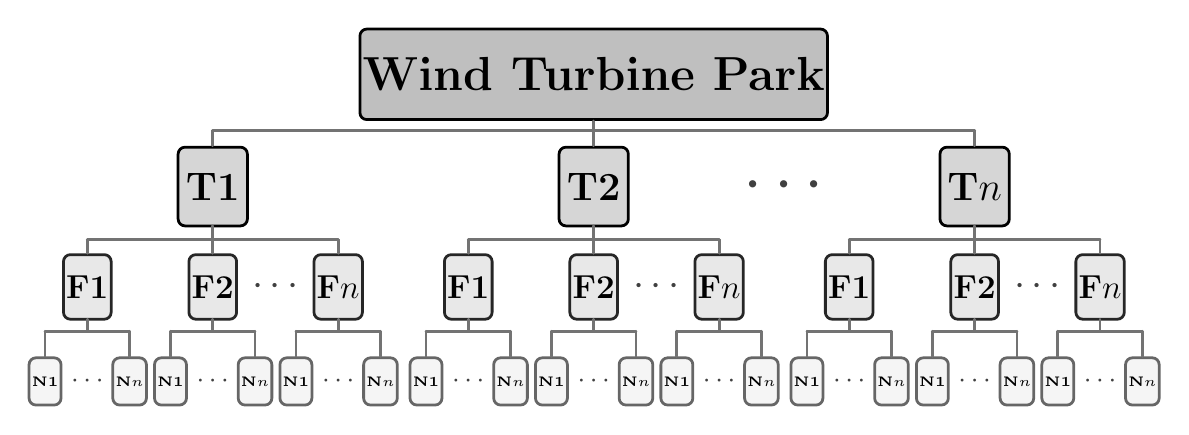
\begin{tikzpicture}[x={\GHx cm}, y=1cm]

\node (park) [parkbox] at (11.81,\Ypark) {Wind Turbine Park};

\foreach \tb/\tl/\tid in {0/1/a, 8.2/2/b, 16.4/{$n$}/c}{

  \node (t\tid) [tbox] at (\tb+3.61,\Yt) {T\tl};

  \node[dots,font=\GHdotsF] (tf\tid)
      at (\tb+4.96,\Yf) {$\cdots$};

  \foreach \fb/\fl/\fid in {0/1/a,2.7/2/b,5.4/{$n$}/c}{

    \node (f\tid\fid) [fbox]
        at (\tb+\fb+0.91,\Yf) {F\fl};

    \node (n\tid\fid a) [ubox]
        at (\tb+\fb,\Yn) {N1};

    \node (n\tid\fid c) [ubox]
        at (\tb+\fb+1.82,\Yn) {N$n$};

    \node[dots,font=\GHdotsN] (nd\tid\fid)
        at (\tb+\fb+0.91,\Yn) {$\cdots$};

    % Flange -> Nuts
    \draw[edge]
      (\tb+\fb+0.91,\Yf-0.41) --
      (\tb+\fb+0.91,\YfBranch);

    \draw[edge]
      (\tb+\fb,\YfBranch) --
      (\tb+\fb+1.82,\YfBranch);

    \draw[edge]
      (\tb+\fb,\YfBranch) --
      (n\tid\fid a.north);

    \draw[edge]
      (\tb+\fb+1.82,\YfBranch) --
      (n\tid\fid c.north);
  }

  % Turbine -> Flanges
  \draw[edge]
      (\tb+3.61,\Yt-0.5) --
      (\tb+3.61,\YtBranch);

  \draw[edge]
      (\tb+0.91,\YtBranch) --
      (\tb+6.31,\YtBranch);

  \draw[edge]
      (\tb+0.91,\YtBranch) --
      (f\tid a.north);

  \draw[edge]
      (\tb+3.61,\YtBranch) --
      (f\tid b.north);

  \draw[edge]
      (\tb+6.31,\YtBranch) --
      (f\tid c.north);
}

\node[dots,font=\GHdotsT]
    (tdots) at (15.9,\Yt) {$\cdots$};

% Park -> Turbines
\draw[edge]
    (park.south) --
    (11.81,\YparkBranch);

\draw[edge]
    (3.61,\YparkBranch) --
    (20.01,\YparkBranch);

\draw[edge]
    (3.61,\YparkBranch) --
    (ta.north);

\draw[edge]
    (11.81,\YparkBranch) --
    (tb.north);

\draw[edge]
    (20.01,\YparkBranch) --
    (tc.north);

\end{tikzpicture}
\end{document}